\documentclass[12pt]{article}

\usepackage{sbc-template}
\usepackage{graphicx,url}
\usepackage[brazil]{babel}   
\usepackage[utf8]{inputenc}
\usepackage{amsmath}

     
\sloppy

\title{Trabalho Prático I \\ Inteligência Artificial (DCC028)}

\author{Hugo Araujo de Sousa \\ (2013007463)}


\address{Departamento de Ciência da Computação \\
	Instituto de Ciências Exatas \\
	Universidade Federal de Minas Gerais
}

\begin{document} 

\maketitle

\section{Introdução}

Em Inteligência Artificial, um tipo particular de agente baseado em objetivo é o \textbf{agente de resolução de problemas} \cite{russell2016artificial}. Esses agentes possuem formulações bem definidas do problema a resolver e consideram como solução para esse problema uma sequência de ações a serem tomadas. Dados um estado inicial e um estado objetivo, esses agentes devem ser capazes de obter uma sequência de ações que os levem do inicial ao objetivo. Esse processo pode ser feito através de uma busca no espaço de estados.

O processo fundamental da busca no espaço de estados é o de analisar o estado atual do agente, obter os estados que podem ser atingidos a partir do estado atual e escolher um deles para seguir, deixando outras opções para mais tarde, caso a opção atual não leve a uma solução. Um exemplo de problema de busca em espaço de estados é o problema de achar uma rota em um determinado ambiente, em que cada posição no ambiente define um estado no espaço. Essas posições podem estar bloqueadas ou livres, permitindo ou não que o agente se movimente por elas, o que torna necessário que o agente seja capaz de decidir qual o melhor caminho a seguir e o que fazer caso encontre posições bloqueadas nesse caminho.

Nesse trabalho, serão implementados algoritmos de busca em espaço de estados, aplicados em um ambiente representado por um mapa de duas dimensões. Os algoritmos serão analisados e comparados, a fim de comparar os caminhos encontrados, o tempo de execução e o número de nodos expandidos no grafo de busca de cada mapa.

\section{Implementação}

Esta seção descreve como a foi feita a modelagem do problema de busca em espaço de estados e as escolhas de implementação realizadas.

\subsection{Mapas} \label{sec:impmap}

Cada mapa passado como entrada dos algoritmos é representado por uma matriz de caracteres. Caracteres ``.'' indicam posições no mapa livres para serem atravessadas pelo agente. Já caracteres ``@'' indicam posições bloqueadas. Os agentes podem se mover em oito direções dentro dos mapas: cima, baixo, direita, esquerda, todas com o custo de 1, e as quatro diagonais, com o custo 1,5. É importante ressaltar que movimentos que levem o agente para fora do mapa de entrada ou que o façam atravessar diagonais em cantos bloqueados não são permitidos, isto é, não é possível seguir um caminho pela diagonal superior direta, por exemplo, caso as posições acima ou à direita do agente estejam bloqueadas.

\subsection{Busca em Grafos}

Ao todo foram implementados 4 algoritmos de busca em espaço de estados, descritos em detalhe na Seção \ref{sec:alg}. Como todos os algoritmos usam o mesmo arcabouço estrutural, com pequenas modificações, a modelagem de dados levou isso em consideração. Dessa forma, implementando todos as estruturas e algoritmos utilizando a linguagem \textit{Python} 3.5, foi definida uma classe \textbf{GraphSearch}, responsável pela implementação da estrutura principal da busca em espaço de estados utilizando grafos. Para isso, também foi necessário implementar a classe \textbf{Node}, que representa um nodo no grafo de busca. Esse nodo guarda informações sobre a posição do mapa que representa, o custo do caminho até essa posição e o nodo anterior a ele no grafo.

A busca em grafos implementada neste trabalho utiliza a versão completa de busca, isto é, o agente evita estados já visitados. Para isso, são mantidas duas listas em memória: a lista \textbf{aberto}, que representa os nodos já visitados, porém, ainda não expandidos, e a lista \textbf{fechado}, que indica quais nodos já foram visitados e expandidos.

\subsection{Algoritmos de Busca} \label{sec:alg}

Uma vez definida a estrutura principal dos algoritmos de busca, 4 algoritmos foram implementados. Eles são descritos a seguir.

\begin{itemize}
	\item \textbf{Busca de aprofundamento iterativo (IDS):} Um dos tipos mais simples de busca em grafos é a busca em profundidade. Com ela, o algoritmo sempre prossegue para o nível mais profundo do grafo (as folhas). À medida que os nodos nos níveis mais profundos são expandidos, a busca volta ao nodo mais profundo que ainda tem sucessores não explorados.

	Um dos principais problemas da busca em profundidade é que ela percorre os maiores caminhos da raiz do grafo até as folhas, quando a solução mais rasa (e de menor custo) pode não estar em um nível tão profundo do grafo de busca. A busca de aprofundamento iterativo resolve esse problema ao executar a busca de profundidade iterativamente, cada vez com um valor limite de profundidade. Essa busca foi implementada na classe \textbf{IDS}, utilizando uma pilha para implementar a lista ``aberto''. A fim de garantir que o algoritmo encontra sempre uma solução ótima ao encontrar uma solução, o conceito de profundidade foi implementado como custo, isto é, à medida que o algoritmo executa, ele não analisará nodos cujo custo atual seja maior do que o custo limite para a iteração atual.

	\item \textbf{Busca de custo uniforme:} Esse tipo de busca expande sempre, dentre os nodos na lista ``aberto'', aquele com o menor custo de caminho \textbf{g(n)}. Para isso, a lista ``aberto'' é implementada como uma fila de prioridade ordenada por \textit{g}. Esse algoritmo está implementado na classe \textbf{UniformCost}.

	\item \textbf{Busca gulosa (best first search):} Esse algoritmo tenta sempre expandir o nodo que está mais próximo do objetivo, pensando que isso levaria a uma solução mais rapidamente. Para isso, a busca avalia os nodos usando simplesmente uma função heurística \textbf{h(n)}, que serve para ordenar a lista ``aberto'' como uma fila de prioridades. Para este trabalho, a heurística desse tipo de busca foi a \textit{Manhattan}, que é calculada dessa forma:

	\begin{align*}
		dx = abs(node.x - goal.x) \\
		dy = abs(node.y - goal.y) \\
		h(n) = (dx + dy)
	\end{align*}

	O algoritmo de busca gulosa está implementado na classe \textbf{BestFirst}.

	\item \textbf{Busca A*:} A busca A* tenta minimizar o custo total estimado da solução. Para isso, avalia não só uma função heurística \textbf{h(n)}, mas também o custo para atingir o nodo \textbf{g(n)} em uma função \textbf{f(n) = g(n) + h(n)}, que ordena a lista ``aberto'' como uma fila de prioridades. Para este trabalho, o algoritmo A* foi implementado com duas possíveis opções de função heurística: a distância \textit{Manhattan}, descrita acima, e a distância \textit{Octile}, que é calculada da seguinte forma:

	\begin{align*}
		dx = abs(node.x - goal.x) \\
		dy = abs(node.y - goal.y) \\
		h(n) = max(dx, dy) + 0.5 * min(dx, dy)
	\end{align*}

	O algoritmo de busca A* está implementado na classe \textbf{AStar}.

\end{itemize}

\subsection{Otimalidade da busca A*} \label{sec:otima}

A otimalidade do algoritmo A* é dependente de algumas características da heurística utilizada. Observemos as duas características a seguir.

\begin{itemize}
	\item \textbf{Heurística Admissível:} Uma heurística é admissível se nunca superestima o custo para atingir um nodo. Isto é, \textit{f(n)} nunca superestima o custo verdadeiro de uma solução ao longo do caminho atual através de \textit{n}.

	\item \textbf{Heurística Consistente:} Uma heurística é consistente se, para todo nodo \textit{n} e todo sucessor \textit{n'} de \textit{n} gerado através de uma ação \textit{a}, o custo estimado para atingir o estado objetivo a partir de \textit{n} nunca é maior que o custo do passo até \textit{n'} mais o custo estimado de se atingir o objetivo a partir de \textit{n'}:

	\begin{align*}
		h(n) \leq c(n, a, n') + h(n')
	\end{align*}

\end{itemize}

De acordo com \cite{russell2016artificial}, a versão de busca em árvore do algoritmo A* é ótima caso a heurística utilizada seja admissível. Já a sua versão de busca em grafo é ótima se a heurística utilizada é consistente. Temos ainda que toda heurística consistente é admissível.

% Manhattan x Octile

Para a distância \textit{Manhattan}, vemos que é fácil provar sua inconsistência, já que:

\begin{itemize}
	\item \textbf{Andando na horizontal ou vertical:} nesse caso, o custo da ação é 1 e o valor da heurística é reduzido ou aumentado em 1 unidade. Logo:

	\begin{align*}
		c(n, a, n') = 1 \\
		h(n') = h(n) \pm 1 \\
		\text{Assim:} \\
		h(n) \leq 1 + (h(n) + 1) \Rightarrow h(n) \leq h(n) + 2 ~ \text{(Ok!)} \\
		h(n) \leq 1 + (h(n) - 1) \Rightarrow h(n) \leq h(n) ~ \text{(Ok!)} 
	\end{align*}

	\item \textbf{Andando nas diagonais:} nesse caso, o custo da ação é 1.5 e o valor da heurística é alterado em $ \pm 2 $ ou $ 0 $. Logo:

	\begin{align*}
		c(n, a, n') = 1.5 \\
		h(n') = h(n) \pm 2 ~ \text{ou} ~ h(n') = h(n) \\
		\text{Assim:} \\
		h(n) \leq 1.5 + h(n) ~ \text{(Ok!)} \\
		h(n) \leq 1.5 + h(n) + 2 \Rightarrow h(n) \leq 3.5 + h(n) ~ \text{(Ok!)} \\
		h(n) \leq 1.5 + h(n) - 2 \Rightarrow 0 \leq -0.5 ~ \text{Impossível!}
	\end{align*}
\end{itemize}

Logo, o algoritmo A* não é ótimo quando utilizando a heurística de distância de \textit{Manhattan} em mapas 2D que permitem movimentos diagonais com custo 1.5.

Analisemos agora a heurística de distância \textit{Octile}.

\begin{itemize}
	\item \textbf{Andando na horizontal ou vertical:} o custo da ação é 1 e o valor da heurística é alterado em $ \pm 0.5 $ ou $ \pm 1 $. Logo:

	\begin{align*}
		c(n, a, n') = 1 \\
		h(n') = h(n) \pm 0.5 ~ \text{ou} ~ h(n') = h(n) \pm 1 \\
		\text{Assim:} \\
		h(n) \leq 1 + h(n) + 0.5 \Rightarrow h(n) \leq h(n) + 1.5 ~ \text{(Ok!)} \\
		h(n) \leq 1 + h(n) - 0.5 \Rightarrow h(n) \leq h(n) + 0.5 ~ \text{(Ok!)} \\
		h(n) \leq 1 + h(n) + 1 \Rightarrow h(n) \leq h(n) \leq h(n) + 2 ~ \text{(Ok!)} \\
		h(n) \leq 1 + h(n) - 1 \Rightarrow h(n) \leq h(n) ~ \text{(Ok!)}
	\end{align*}

	\item \textbf{Andando nas diagonais:} o custo da ação é 1.5 e o valor heurística é alterado em $ \pm 1.5 $ ou $ \pm 0.5 $. Logo:

	\begin{align*}
		c(n, a, n') = 1.5 \\
		h(n') = h(n) \pm 0.5 ~ \text{ou} ~ h(n') = h(n) \pm 1.5 \\
		\text{Assim:} \\
		h(n) \leq 1.5 + h(n) + 0.5 \Rightarrow h(n) \leq h(n) + 2 ~ \text{(Ok!)} \\
		h(n) \leq 1.5 + h(n) - 0.5 \Rightarrow h(n) \leq h(n) + 1 ~ \text{(Ok!)} \\
		h(n) \leq 1.5 + h(n) + 1.5 \Rightarrow h(n) \leq h(n) \leq h(n) + 3 ~ \text{(Ok!)} \\
		h(n) \leq 1.5 + h(n) - 1.5 \Rightarrow h(n) \leq h(n) ~ \text{(Ok!)}
	\end{align*}
\end{itemize}

Portanto, o algoritmo A* é ótimo quando utiliza a heurística de distância \textit{Octile} em mapas 2D que permitem movimentos diagonais com custo 1.5.

\subsection{Entrada, saída e execução}

Os mapas de entrada dos algoritmos devem seguir um formato específico. A primeira linha deve conter o tipo do mapa, as segunda e terceira linhas devem conter a altura e a largura do mapa, respectivamente, e a quarta linha deve conter o nome do mapa. As demais linhas e colunas correspondem à representação do mundo em si (Seção \ref{sec:impmap}).

Como saída, os algoritmos imprimem na saída padrão 4 linhas: a primeira indica o estado inicial; a segunda o estado objetivo; a terceira intencionalmente deixada em branco; e a quarta indica o caminho obtido como solução, começando pelo estado inicial e terminando no estado objetivo, sendo cada estado representado por uma tripla $<$valor\_x, valor\_y, custo$>$. Além disso, uma decisão de implementação que facilitou a visualização dos algoritmos de busca foi a impressão do caminho obtido em um arquivo \textbf{path.map}. Esse arquivo contém o mesmo mapa usado para a busca, entretanto, com três novos caracteres: \textbf{I}, indica a posição inicial do agente; \textbf{F}, indica a posição final do agente; e \textbf{X}, indica uma posição intermediária, pertencente ao caminho solução entre a posição inicial e final do agente.

Para executar os algoritmos de busca, foram criados quatro \textit{scripts}, um para cada algoritmo implementado. São eles: \textbf{aestrela.sh} (A*), \textbf{bg.sh} (busca gulosa), \textbf{ids.sh} (busca de aprofundamento iterativo) e \textbf{ucs.sh} (busca de custo uniforme). Todos os \textit{scripts} recebem, nessa ordem, o nome do mapa a executar a busca, a coordenada \textit{x} do ponto inicial, a coordenada \textit{y} do ponto inicial, a coordenada \textit{x} do ponto final e a coordenada \textit{y} do ponto final. O \textit{script} \textbf{aestrela.sh} recebe, além dos parâmetros citados, um número que indica a heurística a ser utilizada, sendo $ 1 $ referente à heurística de distância \textit{Manhattan} e $ 2 $ referente à heurística de distância \textit{Octile}.

\begin{figure}[htp!]
	\begin{center}
	  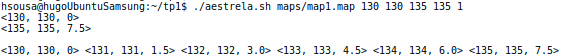
\includegraphics[scale=0.8]{exec.png}
	\end{center}
	\caption{Exemplo de execução do projeto utilizando o algoritmo A* e heurística \textit{Manhattan} no mapa \textbf{map1.map} com ponto inicial (130, 130) e objetivo (135, 135).}
	\label{fig:exec}
\end{figure}

\begin{figure}[htp!]
	\begin{center}
	  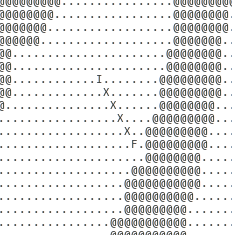
\includegraphics[scale=0.8]{mapex.png}
	\end{center}
	\caption{Representação da solução da execução ilustrada na Figura \ref{fig:exec}.}
	\label{fig:mapex}
\end{figure}

\section{Experimentos}

Esta seção reúne alguns experimentos que foram executados de forma a compreender melhor o comportamento dos algoritmos de busca implementados. Os fatores de interesse escolhidos foram o tempo de execução de cada algoritmo, o custo dos caminhos gerados como solução e o número de nós expandidos por cada algoritmo.

\subsection{Custo dos caminhos}

Para estes experimentos, o algoritmo UCS foi tido como referência principal, uma vez que é um algoritmo ótimo e, dessa forma, o custo da solução encontrada por ele é sempre o menor possível. O algoritmo IDS também poderia ter sido usado como referência, entretanto, seu tempo de execução médio não se mostrou prático, como mostrado na Seção \ref{sec:exptime}.

Para ilustrar o que já foi dito sobre a otimalidade de cada algoritmo, a Tabela \ref{tab:costs} mostra o custo final da solução encontrada pelos algoritmos para o mapa ``map1.map'' com estado inicial (0, 0) e objetivo (247, 245). Podemos notar que as observações sobre otimalidade do algoritmo A* feitas na Seção \ref{sec:otima} são vistas na Tabela.

\begin{table}[htp]
\centering
\begin{tabular}{|l|l|}
\hline
\textbf{Algoritmo} & \textbf{Custo da Solução} \\ \hline
A* Manhattan       & 420                       \\ \hline
A* Octile          & 418.5                     \\ \hline
Busca Gulosa         & 521                       \\ \hline
Custo Uniforme       & 418.5                     \\ \hline
IDS                & 418.5                     \\ \hline
\end{tabular}
\caption{Custo final da solução para cada algoritmo. Mapa ``map1.map'', estado inicial (0, 0) e objetivo (247, 245).}
\label{tab:costs}
\end{table}

\subsection{Nodos expandidos}

\begin{figure}[htp!]
	\begin{center}
	  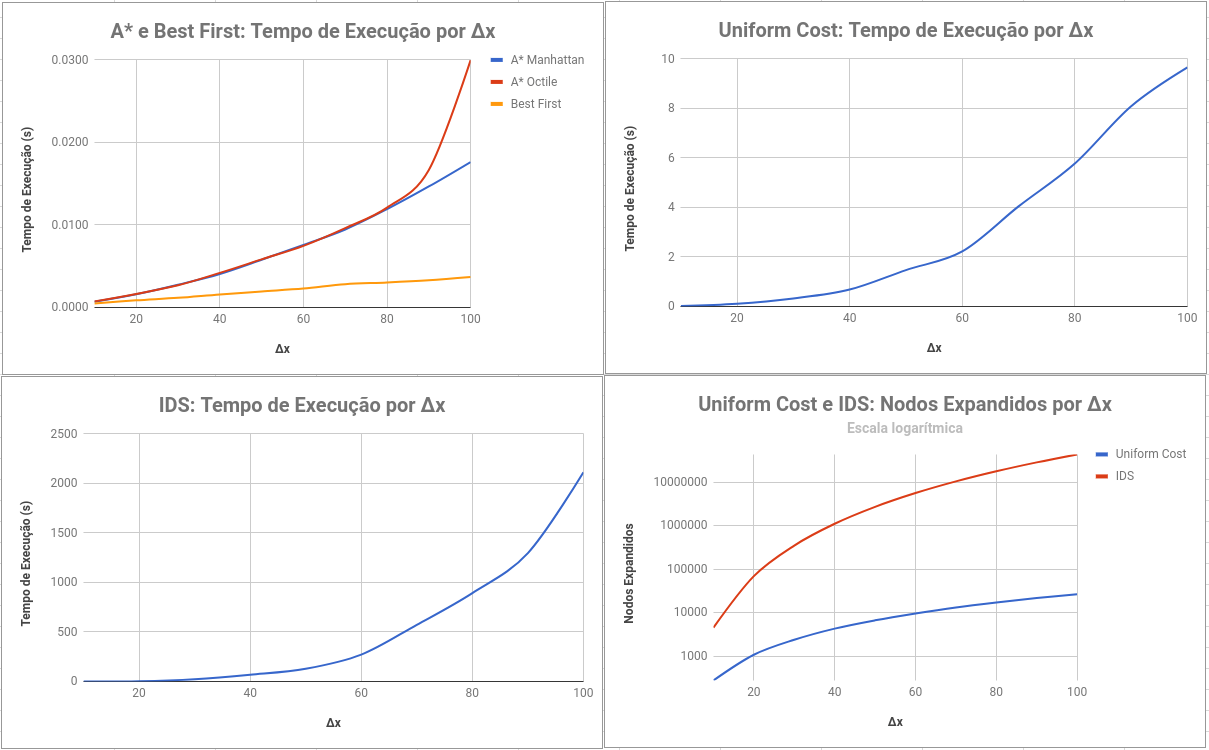
\includegraphics[scale=0.35]{charts.png}
	\end{center}
	\caption{Gráficos de tempo de execução e nodos expandidos para os algoritmos de busca implementados.}
	\label{fig:charts}
\end{figure}

A fim de verificar o comportamento dos algoritmos em relação ao número de nós que expandem e o seus tempos de execução, foi criado um novo mapa, composto apenas por células desbloqueadas. Dessa forma, dado um ponto no inicial no centro do mapa e um ponto objetivo próximo a ele, alterou-se a distância no eixo x entre esses pontos gradualmente, para gerar os gráficos vistos na Figura \ref{fig:charts}.

Chamando a distância no eixo x entre os pontos iniciais e objetivos de $ \Delta x $, temos que, para $ \Delta x = \{10, 20, 30, 40, 50, 60, 70, 80, 90, 100\} $, os algoritmos A* (com ambas as heurísticas) e Busca Gulosa expandiram $ n = \Delta x $ nodos, sendo os mais eficientes em termos de espaço, dentre os algoritmos implementados.

Já os algoritmos Busca de Custo Uniforme e IDS apresentaram um maior número de nodos expandidos, como visto no gráfico do canto inferior direito da Figura \ref{fig:charts}, em escala logarítmica.
Esses resultados são esperados, uma vez que o algoritmo de busca uniforme, no mapa gerado, procura por todos os nodos à sua volta, e o algoritmo IDS faz o mesmo, porém ainda expande mais nodos, uma vez que faz uma busca em profundidade no grafo gerado.

\subsection{Tempo de Execução} \label{sec:exptime}

Os resultados de tempo de execução dos algoritmos são vistos nos gráficos dos cantos superior esquerdo, superior direito e inferior esquerdo da Figura \ref{fig:charts}. Vemos que os algoritmos A* e Busca gulosa, apresentam os menores tempo de execução, o que é uma consequência direta do número de nodos que expandem. Busca gulosa apresenta os menores tempos de execução uma vez que não executam nenhum tipo de cálculo complexo para determinar o próximo nodo a ser expandido.

O algoritmo de busca uniforme executa em tempo praticamente linear, enquanto o algoritmo IDS é exponencial. Vemos que o tempo de execução desse último é o pior de todos, se tornando inviável na prática, para valores de $ \Delta x $ maiores que $ 60 $.

\section{Considerações Finais}

O Trabalho Prático I da disciplina de Inteligência Artificial se mostrou extremamente útil para fixar os conceitos vistos em sala referentes a problemas de busca no espaço de estados. Com ele, foi possível comparar os algoritmos utilizados e entender melhor as vantagens e desvantagens de cada um deles. Além disso, também foi possível visualizar o modo como cada um procura por caminhos no espaço de estados. De maneira geral, as maiores dificuldades durante a implementação do projeto foram o estudo teórico sobre heurísticas e suas propriedades, além da otimalidade do algoritmo A* (Seção \ref{sec:otima}). A implementação do algoritmo IDS também se mostrou mais complicada do que a dos outros algoritmos, uma vez que maiores modificações precisaram ser feitas à estrutura da busca em grafos, usada como classe mãe dos algoritmos.

Também foi possível verificar em quais casos cada algoritmo é mais adequado. Se por um lado o algoritmo A* com heurística Manhattan não retorna sempre uma solução ótima com custos diagonais igual a $ 1.5 $. Entretanto, em mapas como o ``map2.map'', que possuem caminhos mais ou menos horizontais e verticais, ele pode ser mais adequado que o A* com heurística Octile (pois ganha em tempo de execução e tende a retornar soluções ótimas).

\bibliographystyle{sbc}
\bibliography{sbc-template}

\end{document}
